\documentclass[tikz]{standalone}%

\usepackage[utf8]{inputenx}%  http://ctan.org/pkg/inputenx
% Euler for math | Palatino for rm | Helvetica for ss | Courier for tt
\renewcommand{\rmdefault}{ppl}% rm
\linespread{1.05}% Palatino needs more leading
\usepackage[scaled]{helvet}% ss //  http://ctan.org/pkg/helvet
\usepackage{courier}% tt // http://ctan.org/pkg/courier
\usepackage{eulervm}  %  http://ctan.org/pkg/eulervm
% a better implementation of the euler package (not in gwTeX)
\normalfont%
\usepackage[T1]{fontenc}%  http://ctan.org/pkg/fontenc
\usepackage{textcomp}%  http://ctan.org/pkg/textcomp

\usetikzlibrary{patterns}

\begin{document}
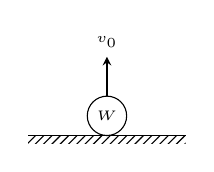
\begin{tikzpicture}
  \draw (0, 0) -- (2cm, 0);

  \fill[pattern = north east lines] (0, 0) rectangle (2cm, -0.1cm);

  \draw (1cm, 0.25cm) circle[radius = 0.25cm] node[font = \tiny] at
  (1cm, 0.25cm) {$W$};
  \draw[-stealth] (1cm, 0.5cm) -- +(0, 0.5cm) node[above, font = \tiny]
  {$v_0$};
\end{tikzpicture}
\end{document}
%%% Local Variables:
%%% mode: latex
%%% TeX-master: t
%%% End:
